\documentclass[12pt,a4paper]{article}
 
                               
\usepackage[T1]{fontenc} % So we can use pretty T1 fonts
\usepackage{libertine}
 
\usepackage[margin=0.5in]{geometry}
\usepackage{amsmath,amssymb,amsfonts}
\usepackage{graphicx}
\usepackage{textcomp}
\usepackage{soul}
\usepackage{hyperref}
\usepackage{xcolor}
\usepackage{caption}
\usepackage{booktabs}
\usepackage{algorithm}
\usepackage{algorithmic}
%\usepackage{helvet}
%\usepackage{courier}
\usepackage{mathtools}
\usepackage{pifont}
\usepackage{dashbox}
\usepackage{xspace}
\usepackage{color}
\usepackage{multirow}
\usepackage{url}
%\usepackage{extsizes}
% the following package is optional:
\usepackage{latexsym}
%\usepackage{mathptmx}
\usepackage{stmaryrd}
\usepackage{enumitem}
\newtheorem{definition}{Definition}
\setlength\parindent{0pt}


\newcommand{\alc}{$\mathcal{ALC}$\xspace}
\newcommand{\el}{$\mathcal{EL}$\xspace}
%para nao ficar o retangulo em volta dos links, apenas muda a cor dos caracteres
\hypersetup{colorlinks,
linkcolor=blue,
filecolor=blue,
urlcolor=blue,
citecolor=blue }

% altera a fonte nas legendas das figuras
%\usepackage[font=small,format=plain,labelfont=bf,up,textfont=times]{caption}
 \newenvironment{problem}[2][{\color{red}Question}]{\begin{trivlist}
\item[\hskip \labelsep {\bfseries #1}\hskip \labelsep {\bfseries #2.}]}{\end{trivlist}}

\newenvironment{problems}[2][{\color{purple}Question}]{\begin{trivlist}
\item[\hskip \labelsep {\bfseries #1}\hskip \labelsep {\bfseries #2.}]}{\end{trivlist}}


\setlength{\parskip}{0,3em}  %altera o espaco entre dois paragrafos
\renewcommand{\baselinestretch}{1.1} %altera o espacamento entre as linhas



\newenvironment{solution}[2][{\color{blue}Model Solution}]{\begin{trivlist}
\item[\hskip\labelsep {\bfseries #1}\hskip \labelsep {\bfseries #2.}]}{\end{trivlist}}

\setlength{\parskip}{0,3em}  %altera o espaco entre dois paragrafos
\renewcommand{\baselinestretch}{1.1} %altera o espacamento entre as linhas
 
\begin{document}


\title{{\color{blue}KRP --- Assignment 2}}
\author{Instructor: Yizheng Zhao}

 
\maketitle

\textbf{$\star$~\textcolor{gray}{This assignment, due on \underline{\textcolor{blue}{21st April at 23:59}}, contributes to 10\% of the final marks for this course. Please be advised that only Questions 1 --- 8 are mandatory. Nevertheless, students can earn up to one bonus mark by completing Question~9. This bonus mark can potentially augment a student's overall marks but is subject to a maximum total of 100 for the course. By providing bonus marks, we aim to incentivize students to excel in their studies and reward those with a remarkable grasp of the course materials.}}

\begin{problem}{{\color{red}1}}
\textbf{Bisimulation Invariance}\\
In the lecture, we defined bisimulation for $\mathcal{ALC}$ and showed bisimulation invariance of $\mathcal{ALC}$ (Theorem 3.2).
\begin{itemize}
    \item Define a notion of ``$\mathcal{ALCN}$-bisimulation'' that is appropriate for $\mathcal{ALCN}$ in the sense that bisimilar elements satisfy the same $\mathcal{ALCN}$-concepts.
    \item Use the definition to show that $\mathcal{ALCQ}$ is more expressive than $\mathcal{ALCN}$.
\end{itemize}
\end{problem}


\begin{problem}{{\color{red}2}}
\textbf{Bisimulation over Filtration}\\
Let $C$ be an $\mathcal{ALC}$-concept, $\mathcal{T}$ an $\mathcal{ALC}$-TBox, $\mathcal{I}$ an interpretation and $\mathcal{J}$ its filtration w.r.t.\ $\textsf{sub}(C)\cup\textsf{sub}(\mathcal{T})$ (see Definition 3.14 for the definition of filtration). Show the truth or falsity of the following statement:
\begin{itemize}
    \item the relation $\rho=\{(\textsf{d}, [\textsf{d}])~|~\textsf{d}\in\Delta^{\mathcal{I}}\}$ is a bisimulation between $\mathcal{I}$ and $\mathcal{J}$.
\end{itemize}
Hint:  If the above relation $\rho$ were a bisimulation, why do we have to explicitly prove Lemma 3.15 in the lecture? Wouldn't Lemma 3.15 then be a consequence of Theorem 3.2?

\end{problem}


\begin{problem}{{\color{red}3}}
\textbf{Bisimulation within the Same Interpretation (2 marks)}\\
We define ``\emph{bisimulations on $\mathcal{I}$}'' as bisimulations between an interpretation $\mathcal{I}$ and itself. Let $\textsf{d},\textsf{e}\in\Delta^{\mathcal{I}}$ be two elements. We write $\textsf{d}\approx_{\mathcal{I}}\textsf{e}$ if they are bisimilar, i.e., if there is a bisimulation $\rho$ on $\mathcal{I}$ such that $\textsf{d}~\rho~\textsf{e}$.
\begin{itemize}
    \item Show that $\approx_{\mathcal{I}}$ is a bisimulation on $\mathcal{I}$.
\end{itemize}
Consider the interpretation $\mathcal{J}$ defined like the filtration, but with $\approx_{\mathcal{I}}$ instead of $\simeq$.
\begin{itemize}
    \item Show that $\rho=\{(\textsf{d}, [\textsf{d}]_{\approx_{\mathcal{I}}})~|~\textsf{d}\in\Delta^{\mathcal{I}}\}$ is a bisimulation between $\mathcal{I}$ and $\mathcal{J}$.
    \item Show that, if $\mathcal{I}$ is a model of an $\mathcal{ALC}$-concept $C$ w.r.t.\ an $\mathcal{ALC}$-TBox $\mathcal{T}$, then so is $\mathcal{J}$.
    \item Why can't we use the previous result to show the finite model property for $\mathcal{ALC}$?
\end{itemize}
\end{problem}


\begin{problem}{{\color{red}4}}
\textbf{Closure under Disjoint Union}\\
Recall Theorem 3.8 from the lecture, which says that the disjoint union of a family of models of an $\mathcal{ALC}$-TBox $\mathcal{T}$ is again a model of $\mathcal{T}$. Note that the disjoint union is only defined for concept and role names.
\begin{itemize}
    \item Extend the notion of disjoint union to individual names such that the following holds: for any family $(\mathcal{I}_{\nu})_{\nu\in\Omega}$ of models of an $\mathcal{ALC}$-knowledge base $\mathcal{K}$, the disjoint union $\biguplus_{\nu\in\Omega}\mathcal{I}_{\nu}$ is also a model of $\mathcal{K}$.
\end{itemize}
\end{problem}


\begin{problem}{{\color{red}5}}
\textbf{Closure under Disjoint Union}\\
Let $\mathcal{K}=\{\mathcal{T}, \mathcal{A}\}$ be a consistent $\mathcal{ALC}$-KB. We write $C\sqsubseteq_{\mathcal{K}}D$ if $C^{\mathcal{I}}\subseteq D^{\mathcal{I}}$ holds for every model $\mathcal{I}$ of $\mathcal{K}$.
\begin{itemize}
    \item Prove that for all $\mathcal{ALC}$-concepts $C$ and $D$ we have $C\sqsubseteq_{\mathcal{K}}D$ iff $C\sqsubseteq_{\mathcal{T}}D$.
\end{itemize}
Hint: Use the modified definition of disjoint union from the previous question.
\end{problem}


\begin{problem}{{\color{red}6}}
\textbf{Finite Model Property (2 marks)}\\
Let $C$ be an $\mathcal{ALC}$-concept that is satisfiable w.r.t. an $\mathcal{ALC}$-TBox $\mathcal{T}$. Show truth or falsity of the following statement: 
\begin{itemize}
    \item for all $m\geq 1$ there is a finite model $\mathcal{I}_{m}$ of $\mathcal{T}$ such that $|C^{\mathcal{I}_{m}}|\geq m$.
    \item Does it hold if the condition ``$|C^{\mathcal{I}_{m}}|\geq m$'' is replaced by ``$|C^{\mathcal{I}_{m}}|=m$''?
\end{itemize}
\end{problem}


\begin{problem}{{\color{red}7}}
\textbf{Unravelling}\\
Draw the unraveling of the following interpretation $\mathcal{I}$ at $d$ up to depth 5, i.e., restricted to $d$-paths of length at most 5 (see Definition 3.21):
\begin{center}
    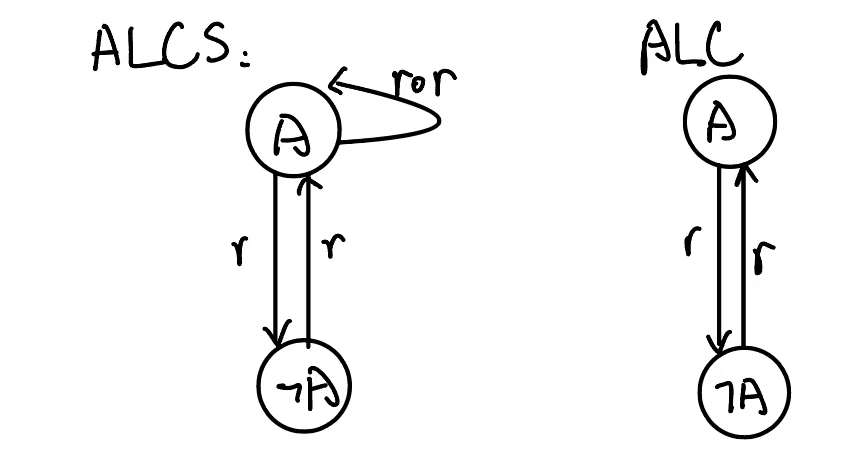
\includegraphics[width=0.22\columnwidth]{4.png}
    \end{center}
\end{problem}


\begin{problem}{{\color{red}8}}
\textbf{Tree Model Property}
\begin{itemize}
    \item Show the truth or falsity of the following statement: if $\mathcal{K}$ is an $\mathcal{ALC}$-KB and $C$ an $\mathcal{ALC}$-concept such that $C$ is satisfiable w.r.t. $\mathcal{K}$, then $C$ has a tree model w.r.t. $\mathcal{K}$.
\end{itemize}
\end{problem}


\begin{problems}{{\color{purple}9 (with 1 bonus mark)}}
\textbf{Bisimulation Invariance}\\
Interpretations of $\mathcal{ALC}$ can be represented as graphs, with edges labeled by roles and nodes labeled by sets of concept names. More precisely, in such a graph:
\begin{itemize}
    \item[] each node corresponds to an element in the domain of the interpretation and it is labeled with all the concept names to which this element belongs in the interpretation;
    \item[] an edge with label $r$ between two nodes says that the corresponding two elements of the interpretation are related by the role $r$.
\end{itemize}
\begin{itemize}
\item Show that: the description logic $\mathcal{S}$ (i.e., $\mathcal{ALC}$ with transitive roles) is more expressive than $\mathcal{ALC}$.
\end{itemize}
\end{problems}



\end{document}
